El desarrollo de la aplicación web presenta grandes desafíos, debido a que en la actualidad existen un gran número de dispositivos móviles y navegadores web con características muy diferentes. Una buena aplicación web es más que algo para mirar, es funcional, interactiva e impecable. A medida que las tecnologías se vuelven inteligentes, debemos ser lo suficientemente inteligentes como para utilizarlas. Con la rápida evolución de las tecnologías web, la complejidad de las aplicaciones web también ha crecido, especialmente al hacer una aplicación web que funcione bien con todas las versiones de todos los navegadores \cite{ochin}.
\vspace{0.8cm}

El desarrollo web es un campo en constante cambio: la forma en que construimos sitios web hoy en día es completamente diferente de cómo solíamos hacerlo hace un par de años. Con la gran cantidad de herramientas disponibles y las nuevas que aparecen todos los días, la mayoría de las veces los desarrolladores se sienten confundidos sobre qué camino tomar.
\vspace{0.8cm}

\subsection{Configuración del entorno de desarrollo}
Los módulos en JavaScript, como en cualquier otro lenguaje de programación, ayudan a descomponer código en partes separadas más pequeñas. Este patrón ayuda a gestionar la creciente complejidad al mantener las preocupaciones separadas en sus partes independientes. En pocas palabras, los módulos ayudan a organizar el código.
\vspace{0.8cm}

Antes de ES6, esto se podía hacer usando diferentes archivos de \gls{script} y luego cargando cada uno de ellos por separado con una etiqueta \code{<script>} en nuestro HTML. Esto tenía muchas desventajas, como mantener el orden correcto de los \gls{script} para evitar romper accidentalmente cualquier código dependiente. Pero afortunadamente, ES6 trajo soporte para módulos con las palabras clave \code{import} y \code{export}, pero aún no son totalmente compatibles en todos los entornos (navegador y Node.js).
\vspace{0.8cm}

Webpack le permite escribir su código en módulos y unificarlos en uno o más paquetes. Webpack permite usar módulos y todas sus bondades sin preocuparse por el soporte. Además de JavaScript, también puede incluir otros tipos de archivos, incluidos (pero no limitados a) CSS, fuentes, imágenes, HTML, etc. y luego transformarlos en un formato aceptable. Webpack es extremadamente potente y se puede ampliar para hacer cosas impresionantes usando el concepto de loaders y \glspl{plugin}.
\vspace{0.8cm}

\subsubsection{Conceptos clave}
Webpack necesita una configuración básica para que funcione debidamente:

\begin{itemize}
  \item Entrada:
  Webpack utiliza el grafo de dependencias para decidir qué módulos deben agruparse. Esto significa que Webpack comienza desde un solo módulo y procesa todas sus dependencias directas e indirectas para formar el grafo de dependencia completo y luego agrupar todos los módulos necesarios.
  El punto de entrada determina desde dónde debe comenzar el paquete web para construir su gráfico de dependencia interna.\\
  Entrada del proyecto: \code{./src/app.js}
  \item Salida:
  La salida determina dónde se supone que el paquete web debe emitir los paquetes que crea y cómo los nombra. Este directorio también contendrá todos los archivos estáticos de la aplicación web que serán visibles al publico mediante el servidor Express.js.\\
  Salida del proyecto: \code{./www/bundle.js}
  \item Loaders
  Los loaders en el paquete web son los que le permiten manejar archivos que no son JavaScript (el empaquetador web solo comprende JavaScript). Los loaders leen varios tipos de archivos y los transforman en módulos válidos que webpack puede entender.
  \item Plugins
  Los \glspl{plugin} son la característica más poderosa de webpack, se utilizan para una amplia gama de tareas que los loaders no pueden realizar. Se utilizan  para la optimización de paquetes, \gls{minificacion}, emisión de estadísticas, etc.
\end{itemize}
\vspace{0.8cm}

\subsubsection{Babel Loader}
Babel ofrece el último soporte de sintaxis ECMAScript (ES5, ES6). Las librerías mas recientes insisten en que se utilicen las últimas ofertas de JavaScript para obtener un código más limpio y legible. Pero desafortunadamente nuestros navegadores no entienden la mayor parte de la sintaxis aquí es donde entra en juego Babel. Es responsable de convertir el código ES5 y ES6 en código comprensible por el navegador, básicamente compatibilidad con versiones anteriores. Las dependencias que necesita el proyecto son las siguientes:
\vspace{0.8cm}

\begin{itemize}
  \item babel-core: El motor principal de Babel para que sus dependientes trabajen.

  \item babel-preset-env: esta es la parte de soporte ES5, ES6

  \item babel-preset-react: Babel se puede usar en cualquier \gls{framework} que necesite el soporte de sintaxis JS más reciente, en este caso es `React'.

  \item babel-loader: Un puente de comunicación entre Webpack y Babel
\end{itemize}
\vspace{0.8cm}

\lstinputlisting[style=ES6, caption=Fragmeno de configuración Babel.]{code/babelrc.json}

\lstinputlisting[style=ES6, caption=Fragmeno de configuración Webpack]{code/webpack.js}

\subsubsection{Webpack Dev Server}
La herramienta Webpack Dev Server ejecuta y sirve una compilación de nuestro proyecto, pero no lo escribe en el disco, lo hace en la memoria. En modo de desarrollo, este modulo hace que la aplicación se abra un navegador, y vuelva a cargar el navegador cuando detecte cambios en los archivos de los que depende la aplicación web.
\vspace{0.8cm}

\lstinputlisting[style=ES6, caption=Configuración Webpack Dev Server.]{code/webpack.dev.js}

Con la ayuda de Webpack se tiene la capacidad de importar estilos y componentes de React y hacer que algo no solo sea funcional, sino también estético. Los procesos de construcción pueden ser desalentadores, pero si se tiene una base sólida y se sabe cómo expandirla, pueden obtenerse buenos resultados.
\vspace{0.8cm}

% \begin{figure}[H]
%   \centering
%   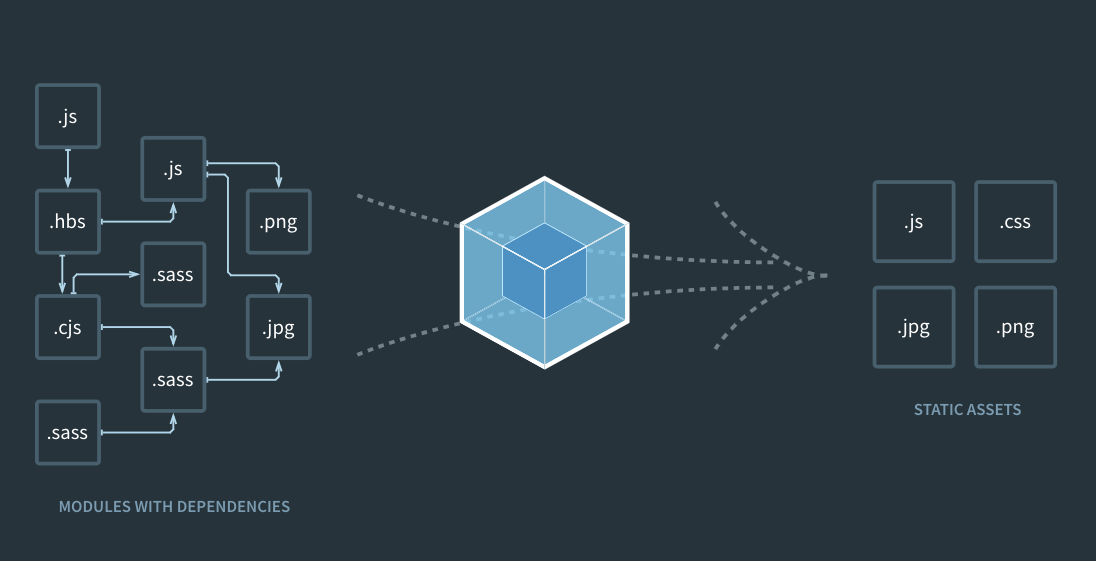
\includegraphics[width=1\textwidth]{webpack}
%   \caption{Imagen de la página oficial de Webpack donde se explica su concepto básico \cite{webpack}.}
% \end{figure}

\subsection{Patrones de diseño}
Las aplicaciones web modernas tienen una estructura de programa compleja, debido a las funcionalidades que proporcionan en sus interfaces de usuario. Escribir manualmente un código de programa puede dar como resultado una calidad y contenido desiguales en partes individuales de la aplicación. Mantener tales aplicaciones desarrolladas es más difícil. Debido a esto, las aplicaciones web a menudo se desarrollan utilizando diferentes \glspl{framework} y patrones de diseño.
\vspace{0.8cm}

Estos esquemas facilitan la reutilización de diseños y arquitecturas exitosas; también ayudan a elegir alternativas de diseño que hacen que un sistema sea reutilizable y evitar alternativas que comprometan la reutilización. Pueden incluso mejorar la documentación y el mantenimiento de los sistemas existentes.
\vspace{0.8cm}
Estos estándares de resolución de problemas pueden ser increíblemente útiles si se usan en las situaciones correctas y por las razones correctas. Cuando se usan estratégicamente, pueden hacer que un programador sea significativamente más eficiente al permitirle el usar métodos refinados por otros y evitar `reinventar la rueda'. También proporcionan un lenguaje común útil para conceptualizar problemas y soluciones repetidos cuando se discute con otros o se maneja el código en equipos más grandes.

\subsection{Redux}
Redux es un administrador de estado predecible para aplicaciones JavaScript basado en el patrón de diseño Flux. A medida que una aplicación crece, se hace difícil mantenerla organizada y mantener el flujo de datos. Redux resuelve este problema administrando el estado de la aplicación con un único objeto global llamado Redux Store. Los principios fundamentales de Redux ayudan a mantener la coherencia en toda la aplicación, lo que facilita la depuración y las pruebas. Redux se puede conectar con cualquier biblioteca de JavaScript. Sin embargo, funciona muy bien con ReactJS debido a su naturaleza funcional.
\vspace{0.8cm}

Redux ayuda a separar el estado de la aplicación, crea un almacén global que reside en el nivel superior de una aplicación y alimenta con el estado a todos los componentes internos. A diferencia de Flux, Redux no tiene múltiples objetos de almacenamiento. El estado completo de la aplicación está dentro de un objeto, y potencialmente podría intercambiar la capa de vista con otra biblioteca con el almacenamiento intacto.

\subsubsection{Redux/Flux}
Redux adoptó un gran número de restricciones de la arquitectura Flux: las acciones encapsulan la información para que el Redux Reducer actualice el estado de manera determinista, el estado es un Redux Store \gls{singleton}. El despachador de Flux único se reemplaza con múltiples Redux Reducers pequeños que recogen información de las acciones y la `reducen' a un nuevo estado que luego se guarda en el Redux Store. Cuando se cambia el estado en el Store, la Vista según la suscripción recibe propiedades llamadas props.
\vspace{0.8cm}

\begin{figure}[H]
  \centering
  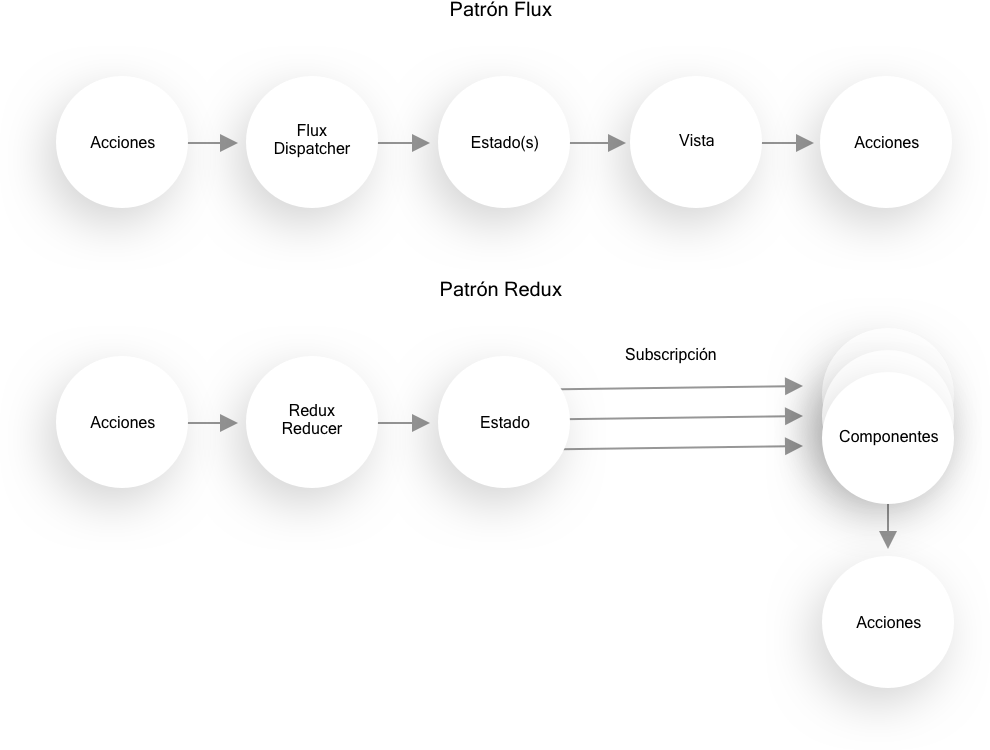
\includegraphics[width=0.9\textwidth]{flux-redux}
  \caption{Comparación Flux/Redux. (Fuente: Elaboración propia)}
\end{figure}
\vspace{0.8cm}

Para trabajar con Redux se necesitan tres cosas:
\begin{itemize}
  \item Actions (acciones): estos son objetos que deben tener dos propiedades, una que describe el tipo de acción y otra que describe lo que se debe cambiar en el estado de la aplicación.

  \item Reducers (reductores): son funciones que implementan el comportamiento de las acciones. Cambian el estado de la aplicación, en función de la descripción de la acción y la descripción del cambio de estado.

  \item Store (almacén): reúne las acciones y los reducers, manteniendo y cambiando el estado de toda la aplicación; solo hay una store.
\end{itemize}

\subsubsection{Redux Store}
Redux Store contiene un objeto del estado global de la aplicación. Esta actualiza el estado y notifica los componentes suscritos.
\vspace{0.8cm}

\lstinputlisting[style=ES6, caption=Fragmento de código para inicializar el Redux Store]{code/redux-store.js}

\subsubsection{Redux Reducer}
Un Redux Reducer es solo una función pura de JavaScript. Recibe dos parámetros: el estado actual y la acción. Una función pura es aquella que devuelve exactamente la misma salida para la entrada dada. El estado es el objeto Redux Store completo, la acción es el objeto despachado con un tipo requerido y un payload opcional.
\vspace{0.8cm}

\lstinputlisting[style=ES6, caption=Fragmento de código del reducer común de la app]{code/redux-reducer.js}

\subsubsection{Acciones Redux}
La única forma de cambiar el estado es enviando una señal al Store. Esta señal es una acción. Entonces "despachar una acción" significa enviar una señal a Redux Store.
\vspace{0.8cm}

\lstinputlisting[style=ES6, caption=Fragmento de una acción que actualiza el estado]{code/redux-action.js}

Este es un modelo conveniente y directo para estructurar datos en una aplicación y presentarlos en el cliente. La aplicación tiene un estado raíz. Un cambio de estado desencadena actualizaciones de vista. Solo las funciones especiales pueden modificar el estado. Una interacción del usuario activa estas funciones especiales de cambio de estado. Solo se produce un cambio a la vez. Esto significa que el estado central no puede desencadenar ninguna otra acción. Solo una entrada del usuario puede desencadenar otra acción \cite{mukhiya}.

\subsection{Integración React/Redux}
Redux practica la teoría de flujo de datos unidireccional y se convirtió en un patrón de facto como tecnología de gestión de estado para aplicaciones ReactJS. React utiliza \textit{props} (abreviatura de propiedades) en un componente que permite el uso de variables no estáticas. Con la ayuda de \textit{props}, podemos pasar estas variables a varios otros componentes (secundarios) desde el componente principal.
\vspace{0.8cm}

La conexión del Store de Redux con los componentes de React, es mediante un componente llamado \code{Provider} del módulo \code{react-redux}. En React para compartir datos entre componentes, un estado tiene que vivir en el componente principal. Este componente principal proporciona un método para actualizar este estado y se pasa como \textit{props} a estos componentes. El único propósito de \code{Provider} es agregar el Store al contexto del componente de la Aplicación, para que todos los componentes secundarios puedan acceder a ella mediante la función \code{connect} de \code{react-redux}. \code{Provider} envuelve a la aplicación React y hace que sea consciente de el Store.
\vspace{0.8cm}

\lstinputlisting[style=ES6, caption=Fragmento de código de la aplicación React principal]{code/redux-react.js}

La función \code{connect} ayuda a conectar un componente con el estado de la aplicación, se debe definir una función especial llamada \code{mapStateToProps} para describir que partes del estado actual de Redux se desean pasar al componente que está envolviendo y una función de nombre \code{mapDispatchToProps} conecta las acciones de Redux con React \textit{props}. De esta manera, un componente React conectado podrá enviar mensajes a el Store.
\vspace{0.8cm}

\lstinputlisting[style=ES6, caption=Ejemplo de conexión de un componente React con el estado Redux]{code/connect.js}
% \begin{enumerate}
%   \item El primer argumento es
% \end{enumerate}

\subsection{Diseño Atómico (Atomic Design)}
El diseño atómico es una metodología compuesta por cinco etapas distintas que trabajan juntas para crear sistemas de diseño de interfaz de una manera más deliberada y jerárquica. Las cinco etapas del diseño atómico son:
\vspace{0.8cm}

\begin{enumerate}
  \item Átomos
  \item Moléculas
  \item Organismos
  \item Plantillas
  \item Páginas
\end{enumerate}
\vspace{0.8cm}

El diseño atómico no es un proceso lineal, sino un modelo mental que nos ayuda a pensar en nuestras interfaces de usuario como un todo cohesivo y una colección de partes al mismo tiempo. Cada una de las cinco etapas juega un papel clave en la jerarquía de nuestros sistemas de diseño de interfaz \cite{frost}.
\vspace{0.8cm}


\begin{figure}[H]
  \centering
  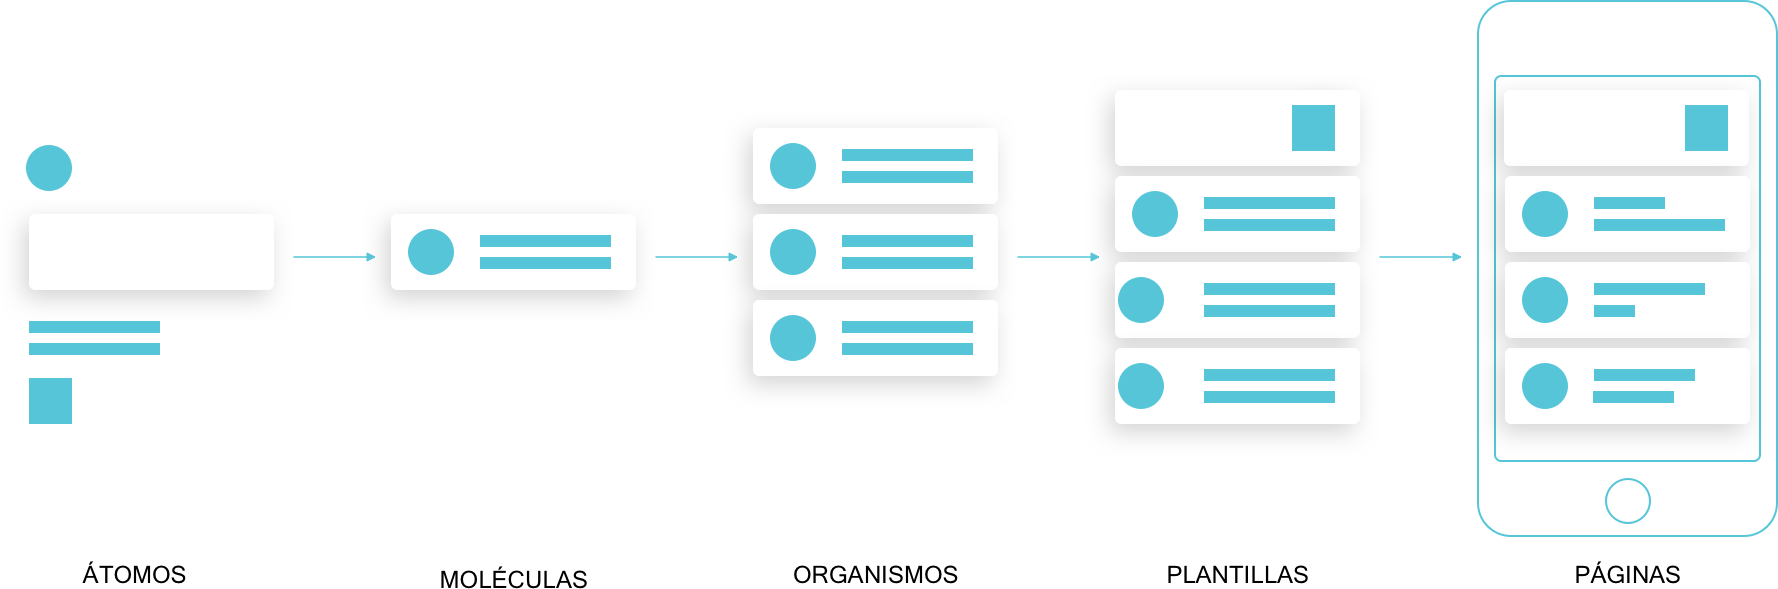
\includegraphics[width=1\textwidth]{atomic}
  \caption{Metodología de diseño atómico. (Fuente: Elaboración Brad Frost 2016)}
\end{figure}

\subsection{Estructura de la aplicación web}
La interfaz de usuario juega un papel muy importante en el aumento de la usabilidad de una aplicación, dado que la IU ofrece al usuario una vista abstracta de todo el sistema, el éxito del sistema depende en gran medida de ello. Por lo tanto, el diseño de la interfaz de usuario debe tener la importancia adecuada en el proceso del ciclo de vida del diseño del sistema.
\vspace{0.8cm}

\subsubsection{Módulo de inicio de sesión}
Uno de los desafíos es cómo implementar un esquema de autenticación y autorización flexible, seguro y eficiente. Parece confuso diferenciar entre autenticación y autorización. De hecho, es muy simple.

\begin{itemize}
  \item Autenticación: se refiere a verificar `quién es usted', por lo que debe usar el nombre de usuario y la contraseña para la autenticación.

  \item Autorización: se refiere a lo que `puede hacer', por ejemplo, acceder, editar o eliminar datos a algunos documentos, esto sucede después de la verificación.
\end{itemize}

Firebase Authentication proporciona servicios de back-end, SDK fáciles de usar y bibliotecas de interfaz de usuario para autenticar a los usuarios en la aplicación. En el código ejemplo \ref{login} se muestran los métodos necesarios para el manejo de sesiones del proyecto.
\vspace{0.8cm}

\lstinputlisting[style=ES6, label=login, caption=Fragmento de código del manejo de sesión de usuario]{code/login.js}

Gracias a la simplicidad y efectividad de los servicios de Firebase, este proceso es utilizado por muchas aplicaciones y servicios web en la actualidad.
\vspace{0.8cm}

\subsubsection{Evaluación de la interfaz de usuario}
El objetivo del proyecto es señalar los problemas y desafíos que surgen del uso de una pantalla táctil como dispositivo de entrada en una aplicación web. Para lograr esto, se desarrolló un prototipo, basado en pautas teóricas. El prototipo fue evaluado en sesiones informales donde los usuarios lo probaron y hablaron sobre cómo lo percibieron. Se alentó a los sujetos a sugerir soluciones alternativas y criticar las soluciones que encontraron negativas.
\vspace{0.8cm}

El prototipo inicial sufrió muy pocos cambios, siendo principalmente por motivos de funcionalidad y no estéticos. Todos los usuarios que sometieron a prueba la aplicación acordaron que el diseño era fácil de entender y se podían acostumbrar a el rápidamente. El resultado de la evaluación demostró que la interfaz responsiva funciona adecuadamente.